% Original vector drawing corresponding to source PDF85, figure16.1.
% All arrows indicate momentum flow; external legs are amputated.
\begingroup
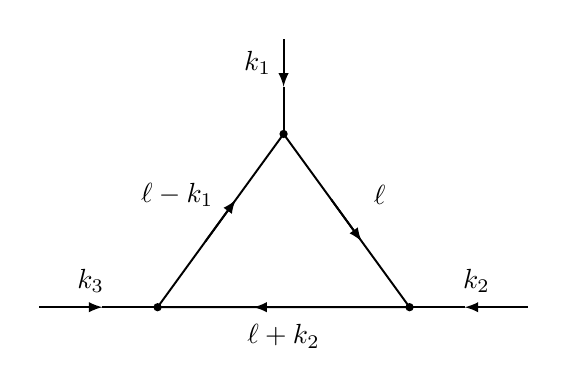
\begin{tikzpicture}[x=1cm,y=1cm,line width=.7pt,>=latex]
\path[use as bounding box] (-3.25,-1.6) rectangle (3.25,2.65);
\coordinate (A) at (0,1.3);
\coordinate (B) at (1.6,-.9);
\coordinate (C) at (-1.6,-.9);
\draw (A)--(B)--(C)--cycle;
\draw[->] (.608,.464)--(.992,-.064);
\draw[->] (.384,-.9)--(-.384,-.9);
\draw[->] (-.992,-.064)--(-.608,.464);
\draw[->] (0,2.5)--(0,1.9);
\draw (0,1.9)--(A);
\draw[->] (3.1,-.9)--(2.3,-.9);
\draw (2.3,-.9)--(B);
\draw[->] (-3.1,-.9)--(-2.3,-.9);
\draw (-2.3,-.9)--(C);
\fill (A) circle[radius=1.5pt];
\fill (B) circle[radius=1.5pt];
\fill (C) circle[radius=1.5pt];
\node at (-.33,2.2) {$k_1$};
\node at (2.45,-.57) {$k_2$};
\node at (-2.45,-.57) {$k_3$};
\node at (1.22,.53) {$\ell$};
\node at (-1.35,.53) {$\ell-k_1$};
\node at (0,-1.27) {$\ell+k_2$};
\end{tikzpicture}
\endgroup

